% ----------------------------------------------------------------------------------
% --------------------------------- 2 NU BETA BETA ---------------------------------
% ----------------------------------------------------------------------------------
\newpage
\section{Analysis of~\texorpdfstring{$2\nu\boldsymbol{\beta}\boldsymbol{\beta}$}{2nu beta beta} data}
\label{sec:2nubb-data}

The latest step of this analysis involves testing all the deep learning models discussed so far with data that are well-known \ac{SSE}-like events. In particular, physics data from period \textit{p03} to period \textit{p09} of \textit{prl25} have been selected for the V08682A detector. Data are categorized by the \texttt{pygama} pipeline according to whether they qualify as $2\nu\beta\beta$ candidates or not in the range between $560$~keV and $2039$~keV\footnote{Below 556 keV, the spectrum is dominated by~${}^{39}$Ar events.}. On top of that, quality cuts listed in Tab.~\ref{tab:quality-cuts-2nu} have been applied.

\begin{table}[H]
    \centering
    \begin{tabular}{ll}
        \toprule
        \textbf{Cut} & \textbf{Filtered events} \\
        \midrule
        detector usability      & events recorded while the detector is not flagged as usable (\texttt{usability} $\neq$ \texttt{on}) \\
        $\beta\beta$-like       & events not flagged as $\beta\beta$-like by the event-level quality selection \\
        good channel            & hits from channels not flagged as good \\
        muon veto               & events in coincidence with a muon \\
        pulser / forced trigger & pulser events and forced-trigger events \\
        \bottomrule
    \end{tabular}
    \caption{Summary of the quality cuts applied to the physics data in the selection of $2\nu\beta\beta$ events.}
    \label{tab:quality-cuts-2nu}
\end{table}

Moreover, data have been cut on the basis of the \ac{lar} veto, as shown in Fig.~\ref{fig:2nu-beforeafterLAR}.
\begin{figure}[H]
    \centering
    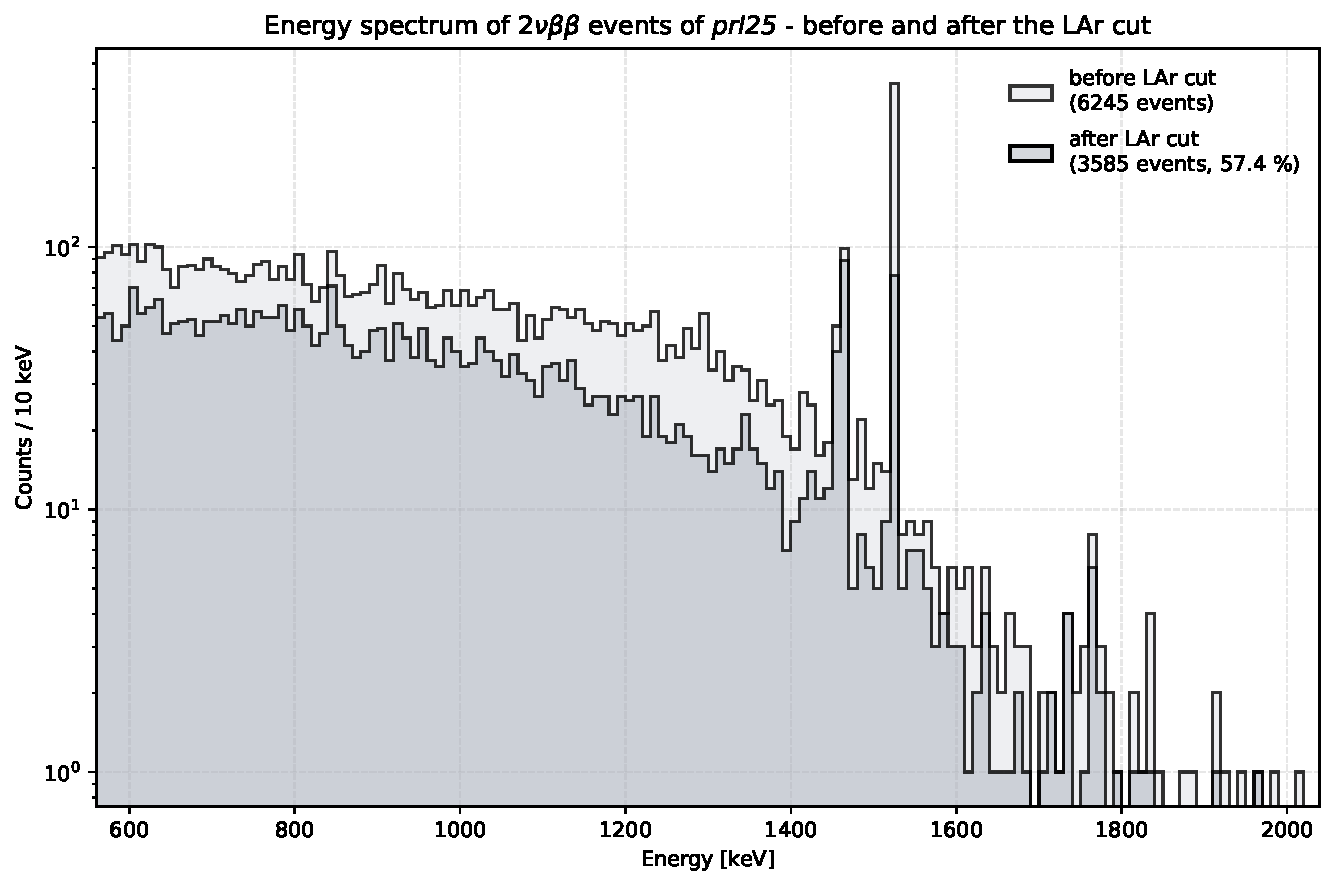
\includegraphics[width=0.8\textwidth]{plots/DTC/2nuData/energy_spectrum_before_after_LAr.pdf}
    \caption{Energy spectrum of the $2\nu\beta\beta$ data before (light grey) and after (dark grey) the \ac{lar} cut.}
    \label{fig:2nu-beforeafterLAR}
\end{figure}
 After the \ac{lar} and muon vetoes, the spectrum between 560 and 2039 keV is dominated by $2\nu\beta\beta$ decays of ${}^{76}$Ge, whose two electrons deposit their energy within a few millimetres and therefore produce \ac{SSE}-like signals. The resulting sample is, however, enriched in SSE-like events rather than pure. $\gamma$-induced events survive the vetoes whenever no energy is deposited in the \ac{lar}, as for the full-energy peaks of ${}^{40}$K (1460.8 keV) and ${}^{42}$K (1524.6 keV), together with part of the underlying Compton continuum. Moreover, a small fraction of genuine $2\nu\beta\beta$ events is itself multi-site because of bremsstrahlung photons emitted by the electrons. The fraction of events retained by a PSD method is therefore expected to be high but not 100\%. Therefore, all of the models discussed in Chapter~\ref{chapter:ML-PSD} and trained on calibration data have been all applied to this novel dataset, without any further training, to test wheter they recognise $2\nu\beta\beta$ events as signal-like or not.

\subsection{\texorpdfstring{\acs{VAE}}{VAE}-based classifier}

\subsection{\texorpdfstring{\acs{DTC}}{DTC}}

% \begin{figure}[H]
%     \centering
%     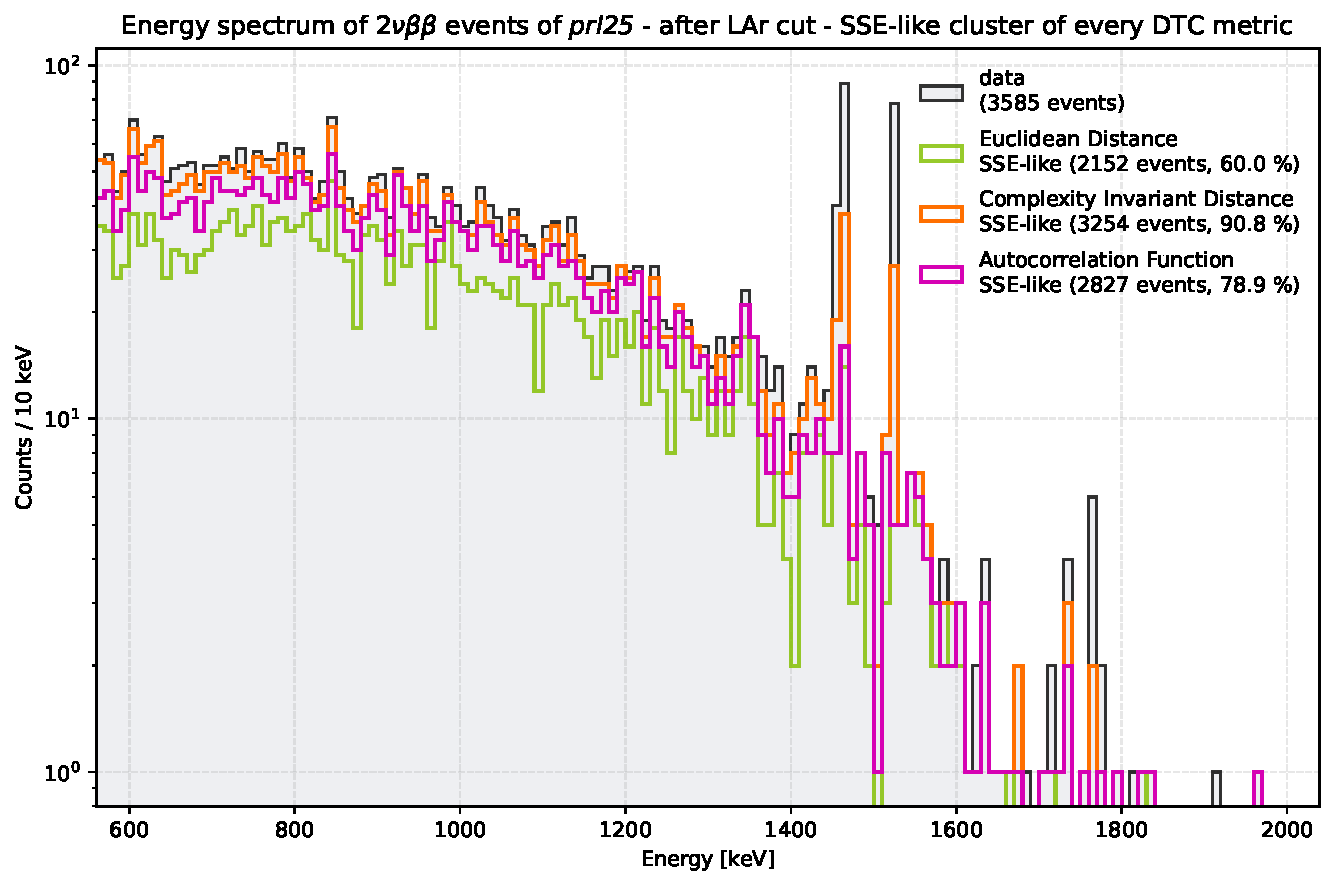
\includegraphics[width=0.8\textwidth]{plots/DTC/2nuData/energy_spectrum_SSE_comparison_afterLAr.pdf}
%     \caption{\ac{DTC} cuts on the $2\nu\beta\beta$ spectrum.}
%     \label{fig:2nu-DTCcus-allmetrics}
% \end{figure}


% \begin{figure}[H]
%     \centering
%     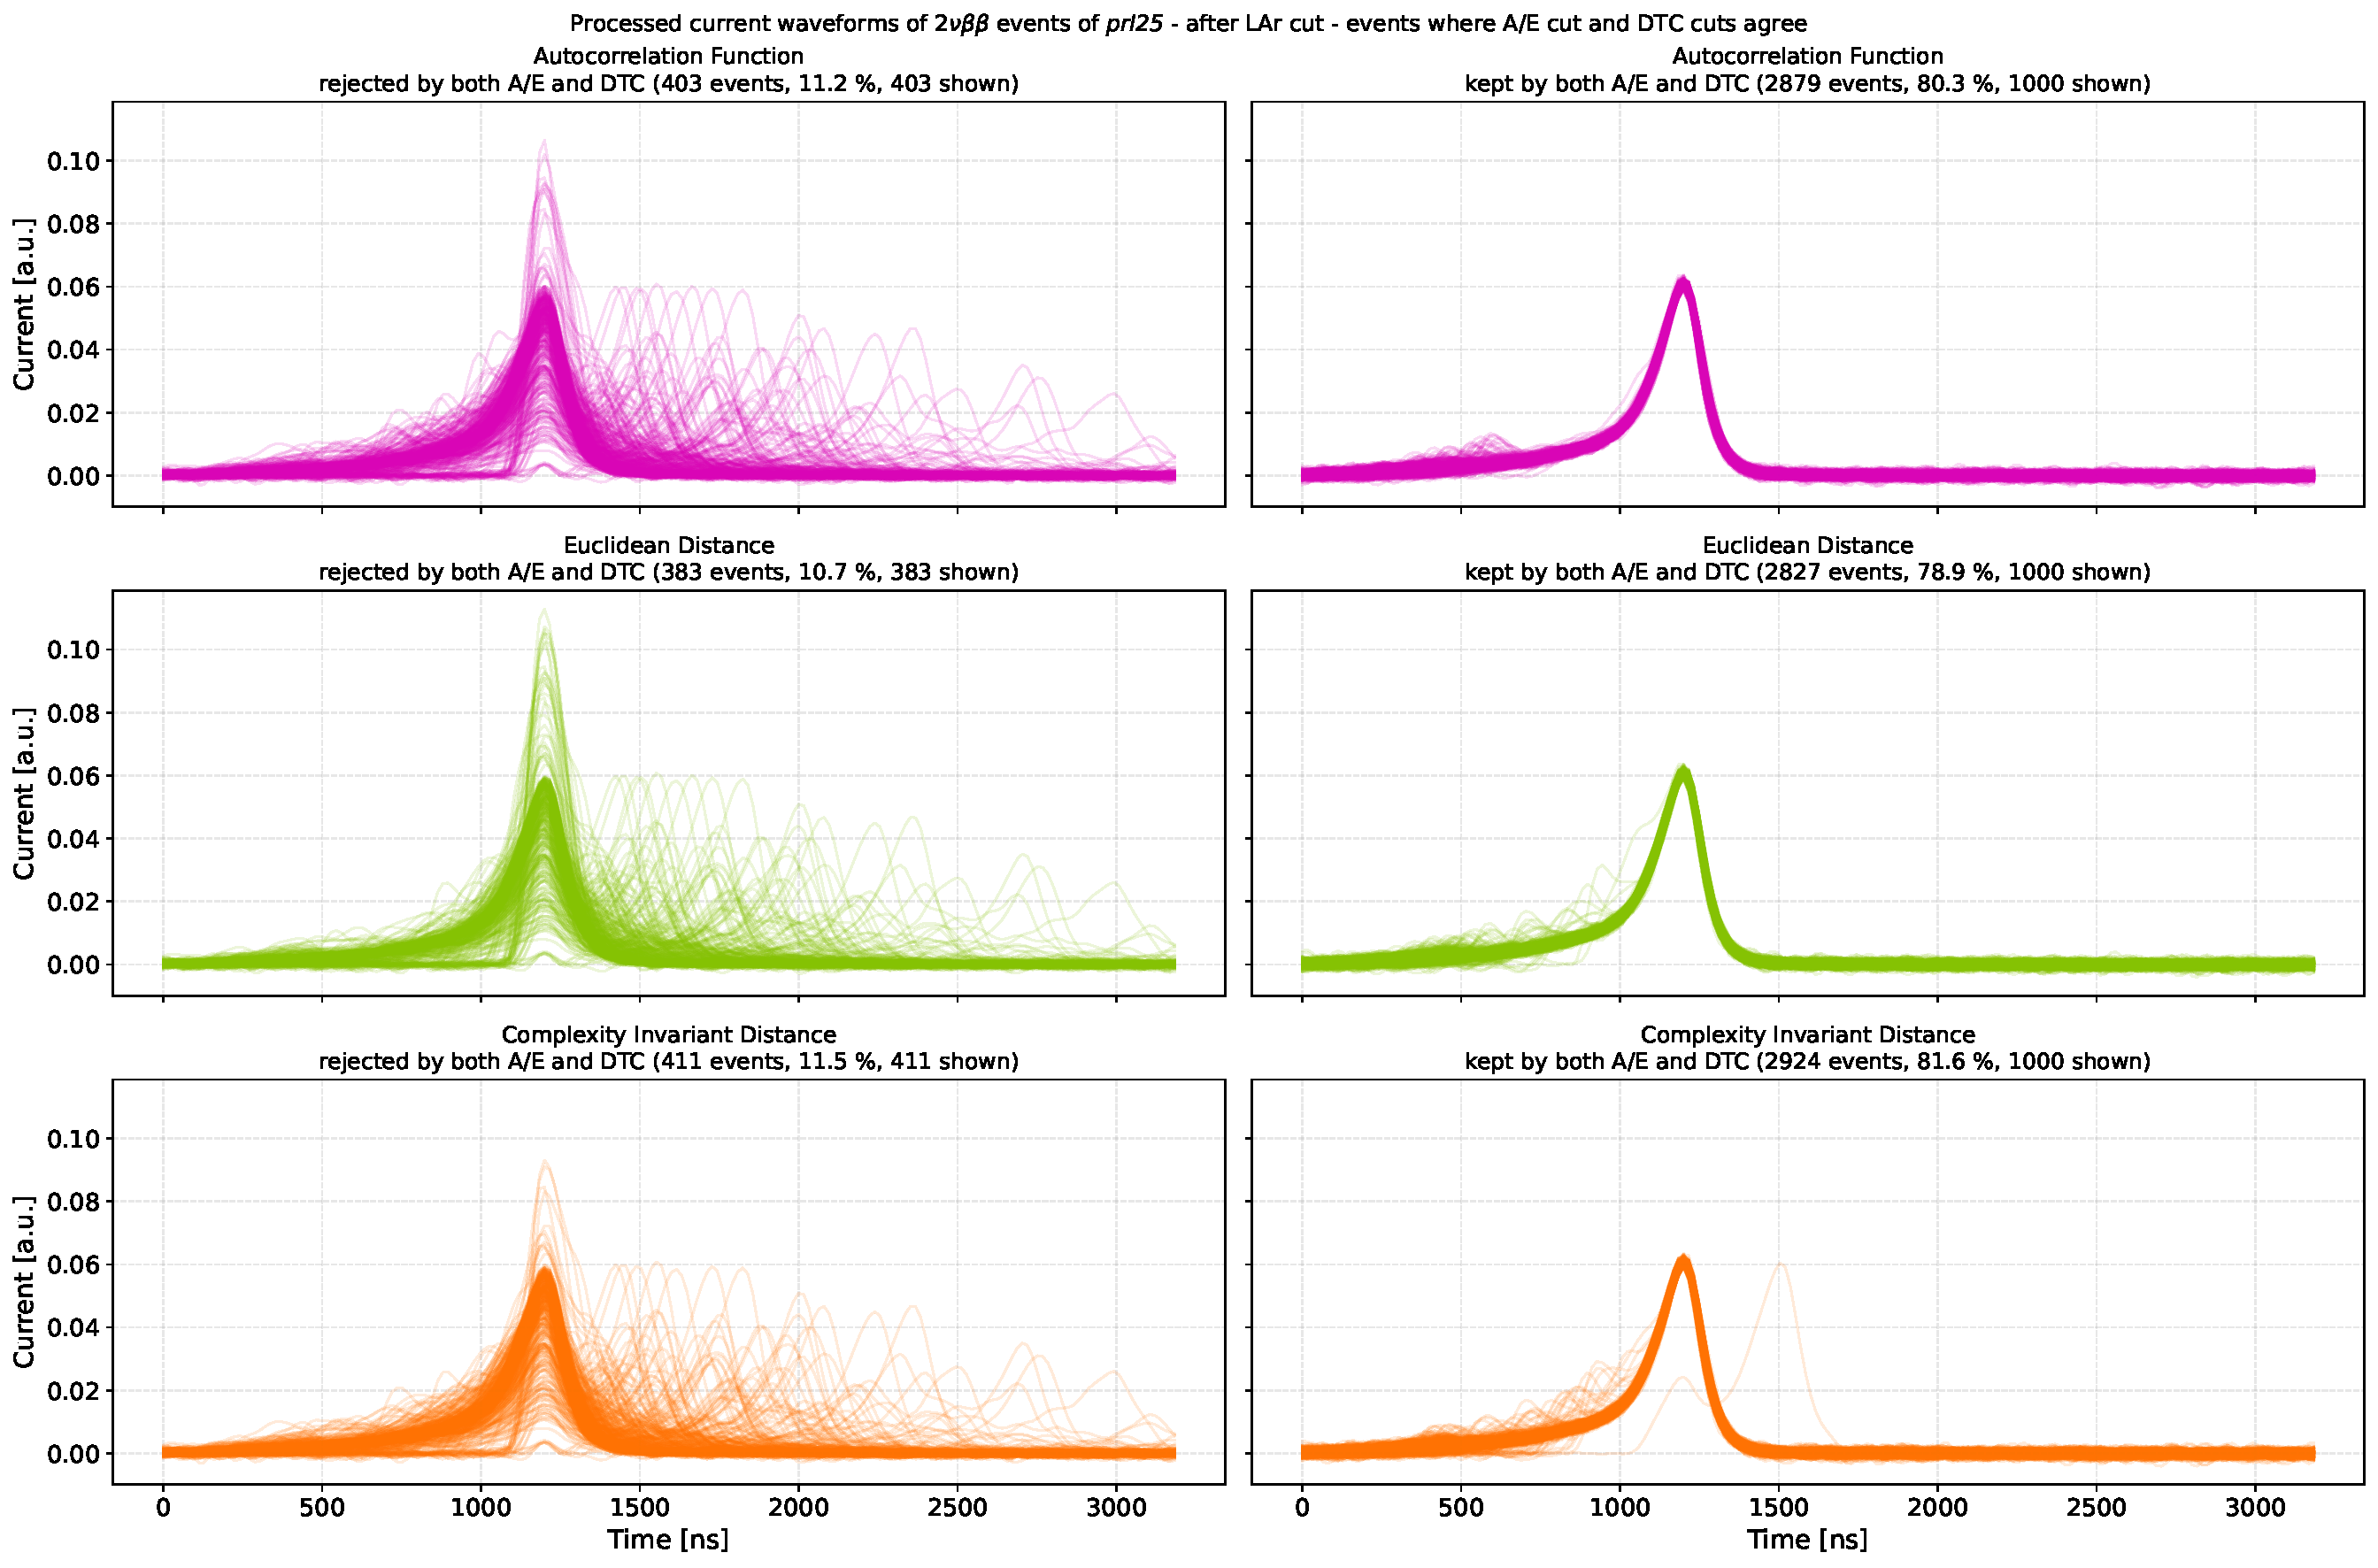
\includegraphics[width=\textwidth]{plots/DTC/2nuData/waveforms_AoE_DTC_agree_afterLAr.pdf}
%     \caption{Waveforms from the $2\nu\beta\beta$ dataset for which the \ac{AE} and the \ac{DTC} agree.}
%     \label{fig:2nu-kept_rejected_AE_DTC_agree}
% \end{figure}

% \begin{figure}[H]
%     \centering
%     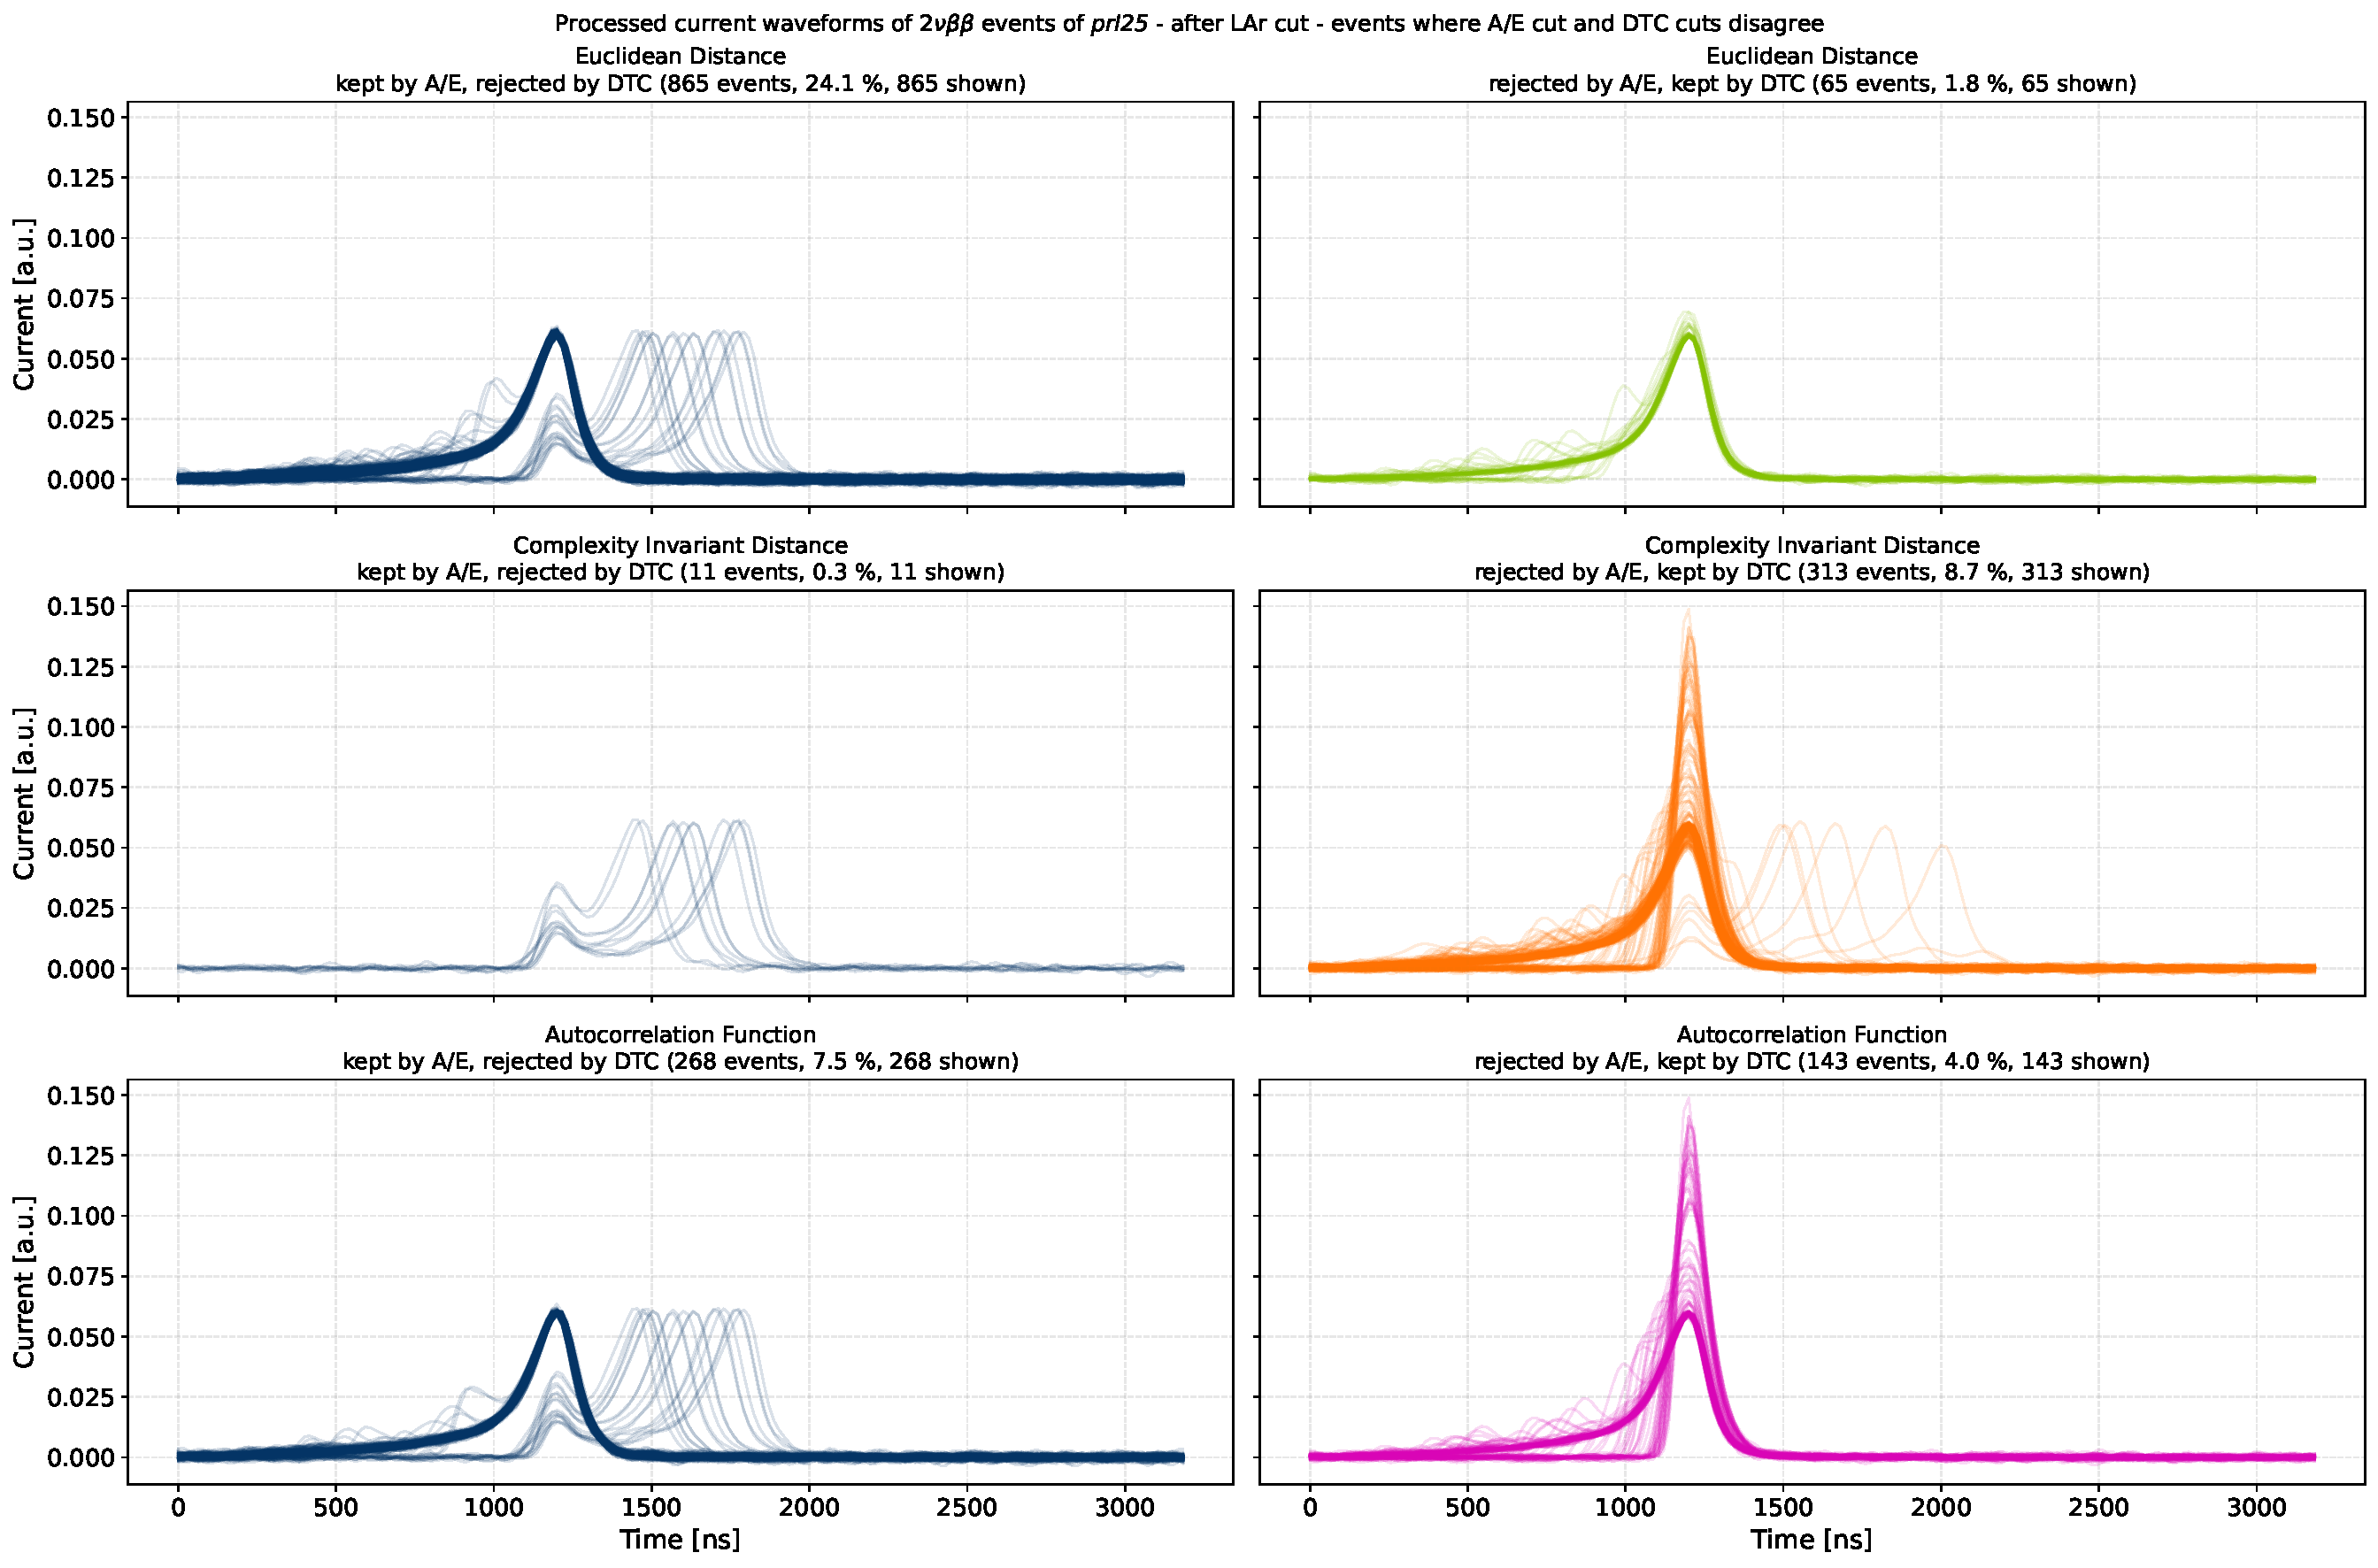
\includegraphics[width=\textwidth]{plots/DTC/2nuData/waveforms_AoE_DTC_disagree_afterLAr.pdf}
%     \caption{Waveforms from the $2\nu\beta\beta$ dataset for which the \ac{AE} and the \ac{DTC} disagree.}
%     \label{fig:2nu-kept_rejected_AE_DTC_disagree}
% \end{figure}

% \begin{figure}[H]
%     \centering
%     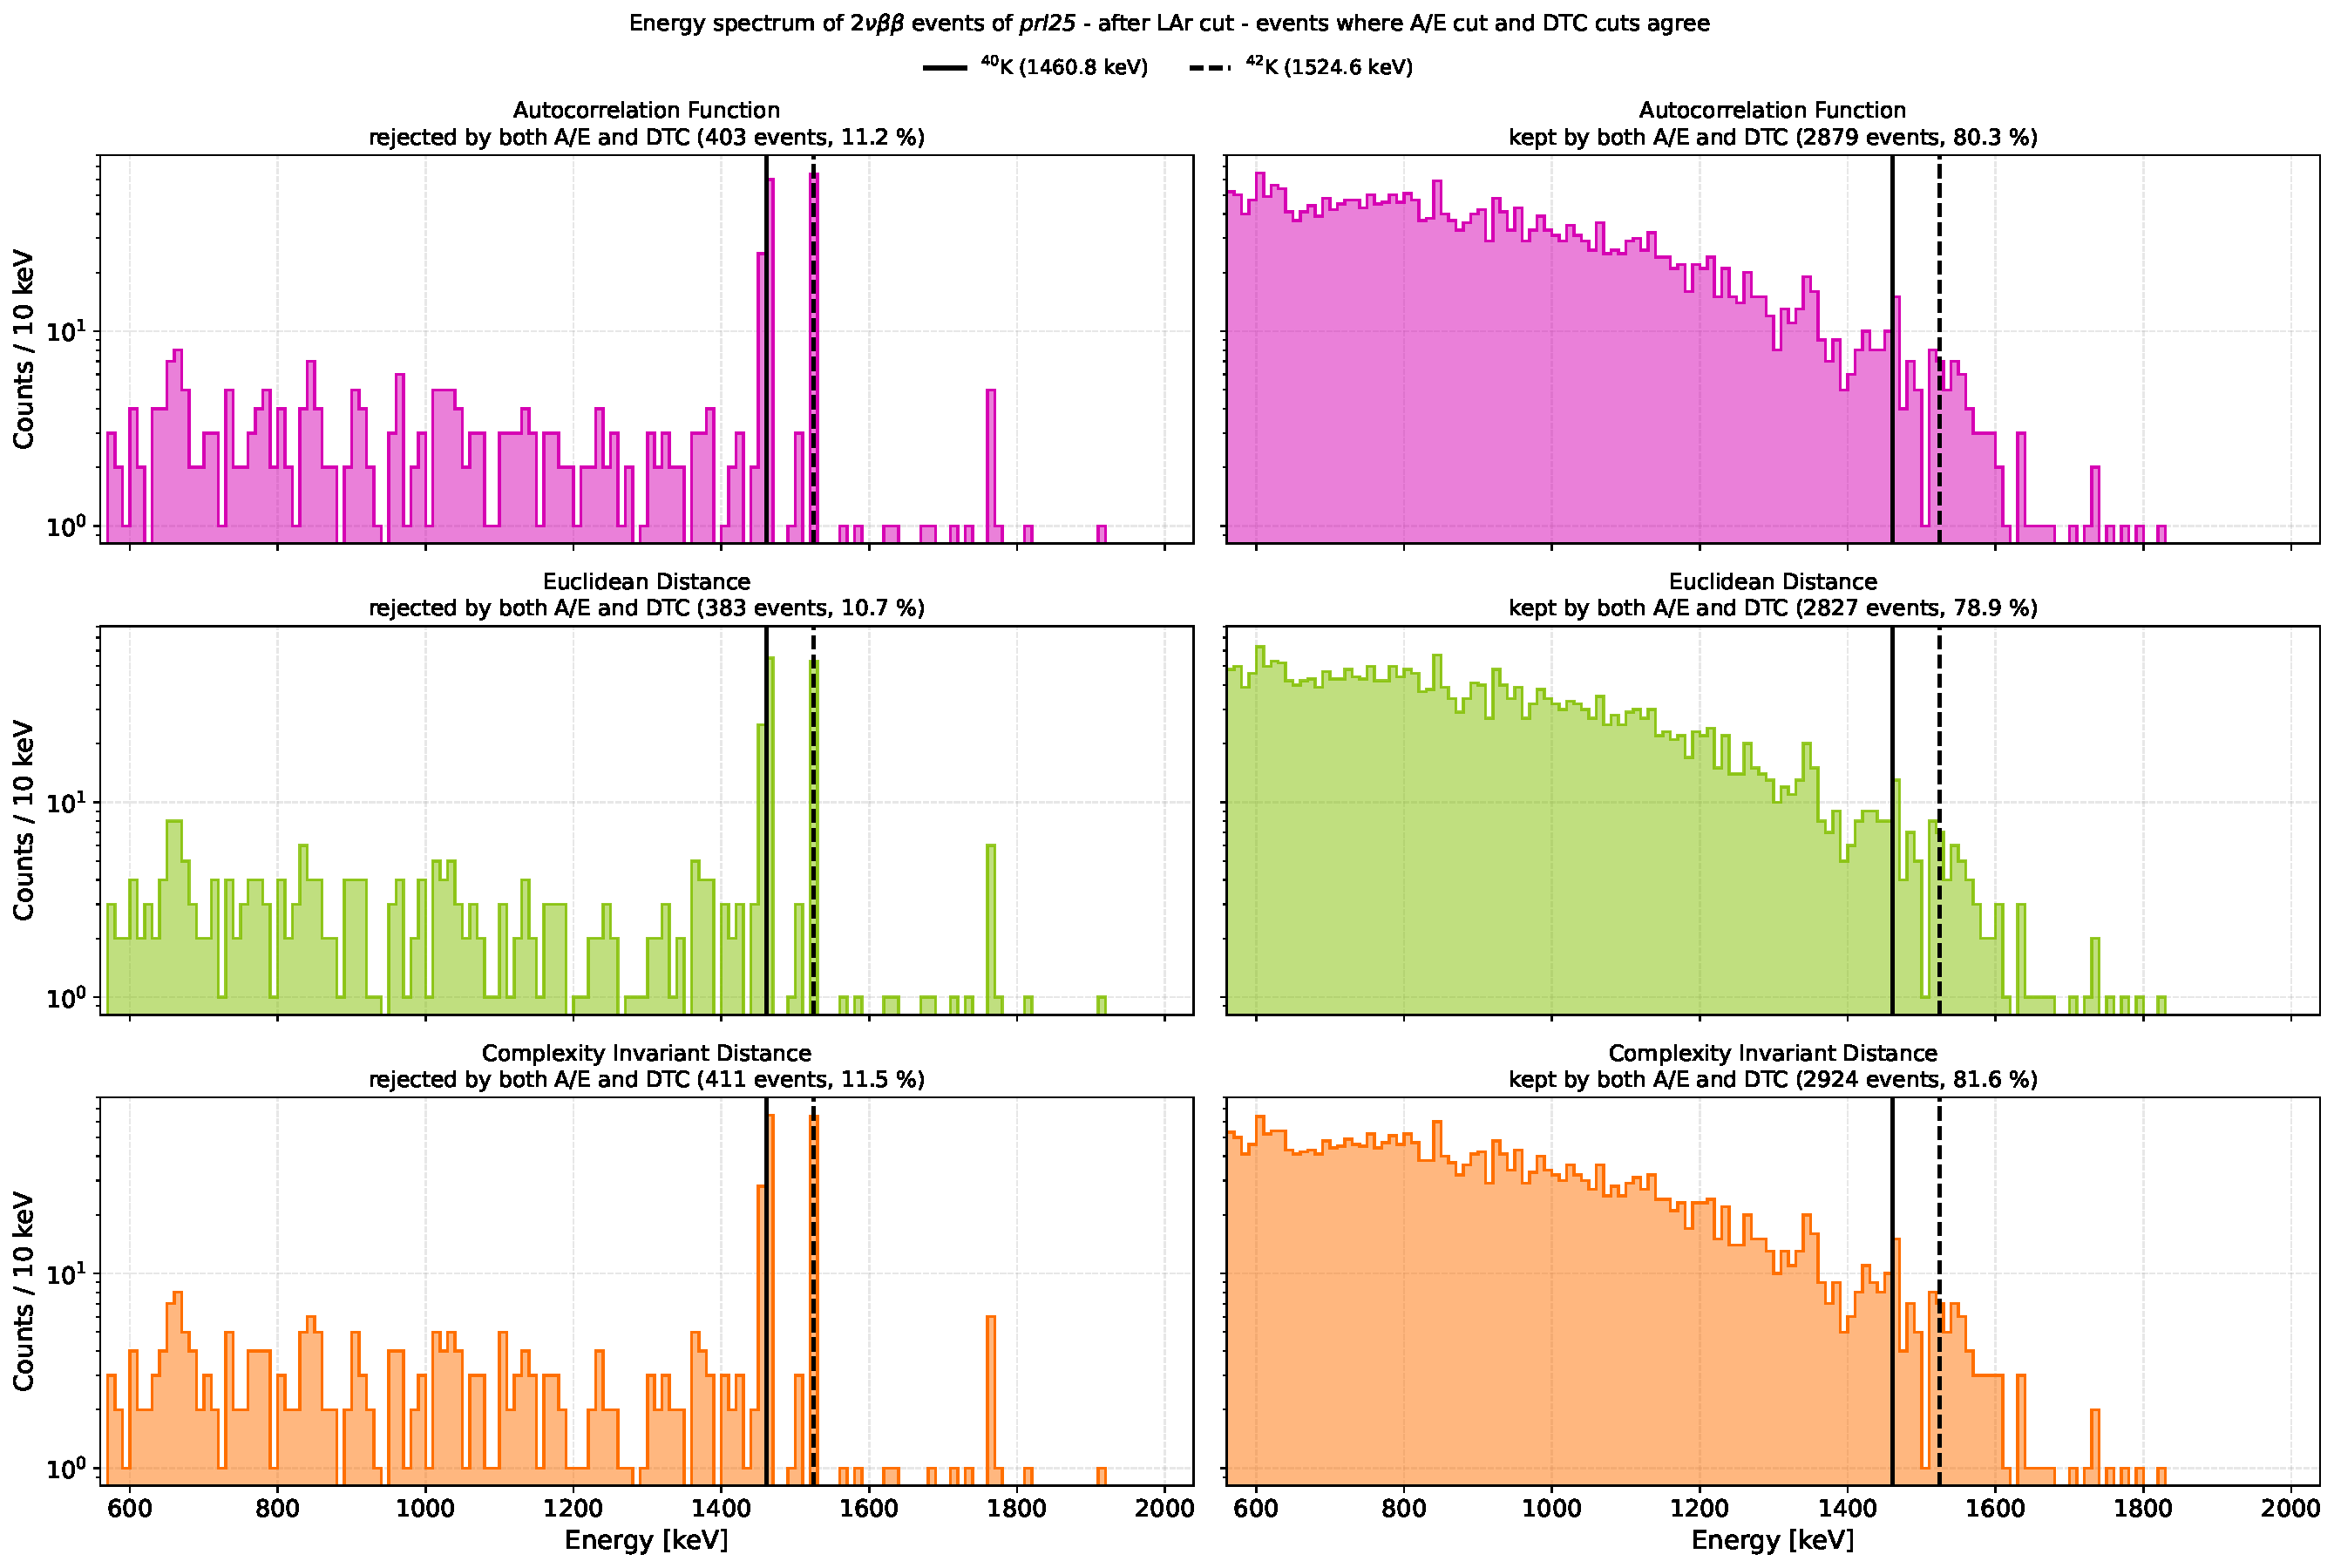
\includegraphics[width=\textwidth]{plots/DTC/2nuData/energy_spectrum_AoE_DTC_agree_afterLAr.pdf}
%     \caption{Energy spectrum of events kept (right) and rejected (left) by both the \ac{AE} cut and the \ac{DTC} algorithm. From the top to the bottom \ac{ACF}, \ac{EUC} and \ac{CID}.}
%     \label{fig:2nu-kept_rejected_AE_DTC_agree_energy}
% \end{figure}

% \begin{figure}[H]
%     \centering
%     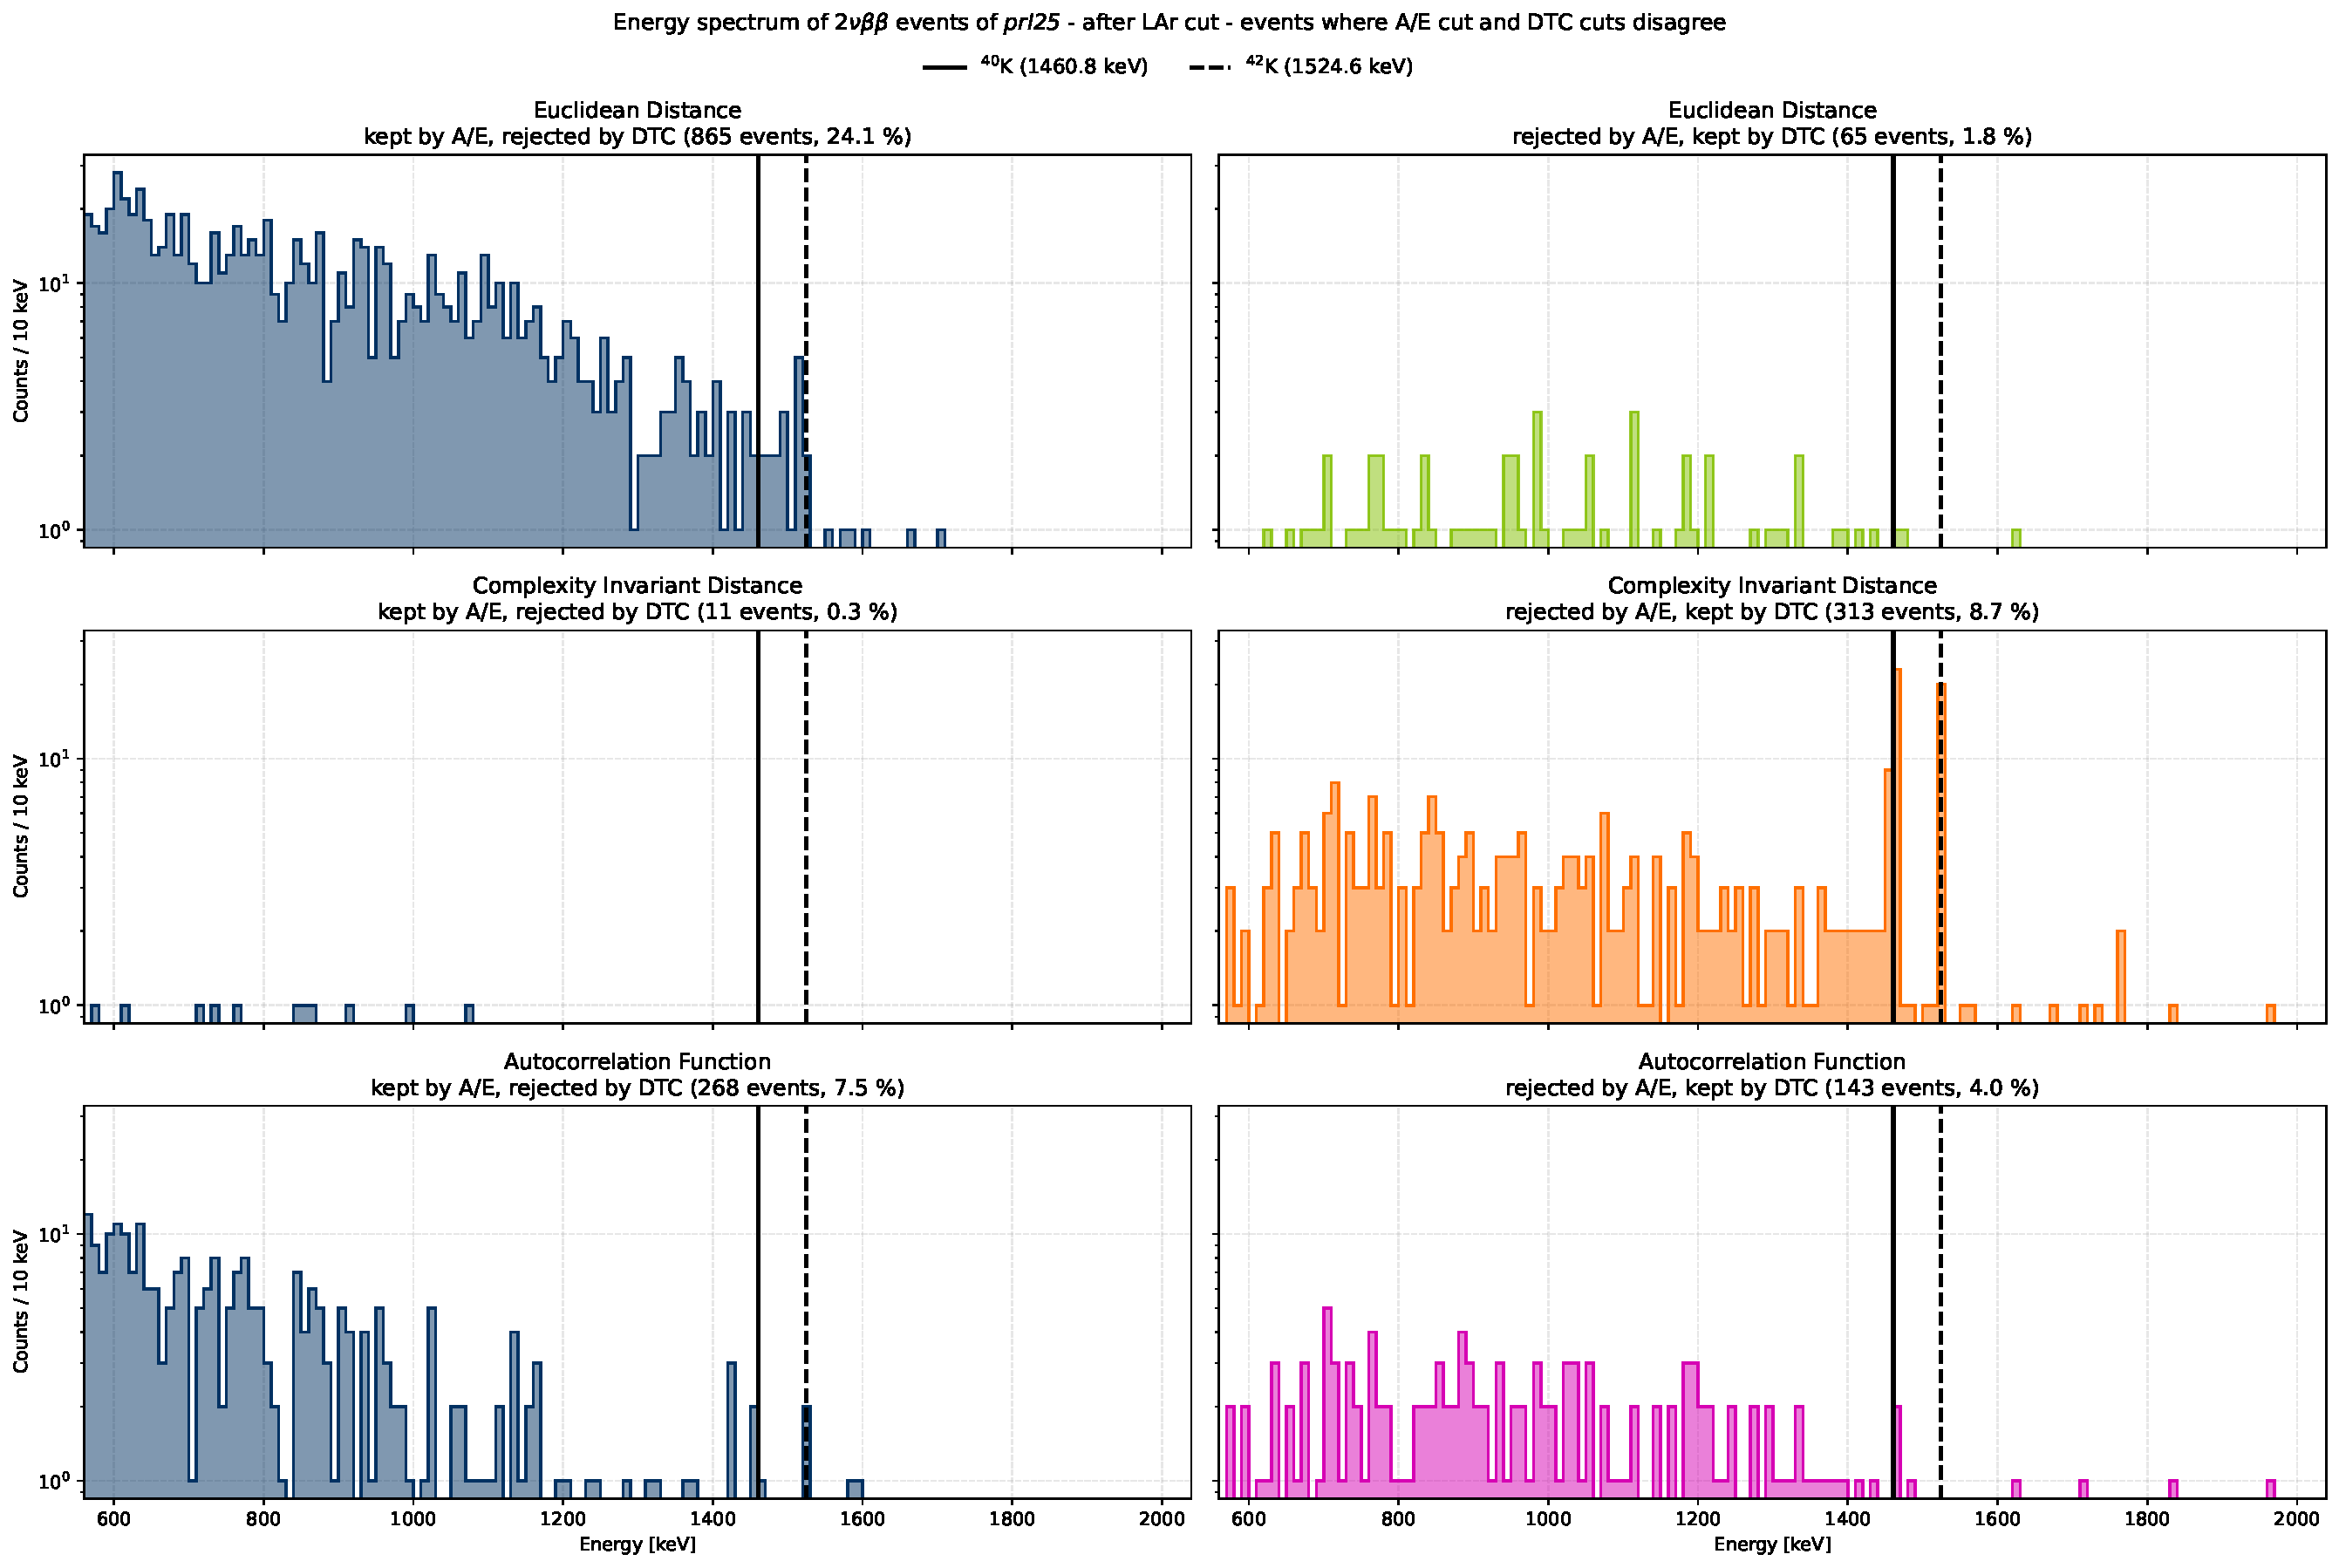
\includegraphics[width=\textwidth]{plots/DTC/2nuData/energy_spectrum_AoE_DTC_disagree_afterLAr.pdf}
%     \caption{Energy spectrum of events kept and rejectd by different cuts: On th eleft waveforms kept by the \ac{AE} cut but rejected by a specific \ac{DTC} metric cut, viceversa on the right events rejected by the \ac{DTC} metric but kept by \ac{AE} are shown. From the top to the bottom \ac{ACF}, \ac{EUC} and \ac{CID}.}
%     \label{fig:2nu-kept_rejected_AE_DTC_disagree_energy}
% \end{figure}